\documentclass[10pt]{article}
\usepackage{float}
\usepackage{amsmath}
\usepackage{paralist}
\usepackage{setspace}
\usepackage{listings}
\usepackage{graphicx}
\usepackage[english]{babel}
\usepackage{geometry}
\usepackage{subcaption}
\usepackage[utf8]{inputenc}
\usepackage{listings}
\usepackage{color}
\usepackage{subcaption}
\usepackage{hyperref}


\begin{document}


\definecolor{mygreen}{rgb}{0,0.6,0}
\definecolor{mygray}{rgb}{0.5,0.5,0.5}
\definecolor{mymauve}{rgb}{0.58,0,0.82}

\lstset{ %
  backgroundcolor=\color{white},   % choose the background color; you must add \usepackage{color} or \usepackage{xcolor}
  basicstyle=\footnotesize,        % the size of the fonts that are used for the code
  breakatwhitespace=false,         % sets if automatic breaks should only happen at whitespace
  breaklines=true,                 % sets automatic line breaking
  captionpos=b,                    % sets the caption-position to bottom
  commentstyle=\color{mygreen},    % comment style
  deletekeywords={...},            % if you want to delete keywords from the given language
  escapeinside={\%*}{*)},          % if you want to add LaTeX within your code
  extendedchars=true,              % lets you use non-ASCII characters; for 8-bits encodings only, does not work with UTF-8
  frame=tb,	                   % adds a frame around the code
  keepspaces=true,                 % keeps spaces in text, useful for keeping indentation of code (possibly needs columns=flexible)
  keywordstyle=\color{blue},       % keyword style
  language=Octave,                 % the language of the code
  otherkeywords={*,...},           % if you want to add more keywords to the set
  numbers=left,                    % where to put the line-numbers; possible values are (none, left, right)
  numbersep=5pt,                   % how far the line-numbers are from the code
  numberstyle=\tiny\color{mygray}, % the style that is used for the line-numbers
  rulecolor=\color{black},         % if not set, the frame-color may be changed on line-breaks within not-black text (e.g. comments (green here))
  showspaces=false,                % show spaces everywhere adding particular underscores; it overrides 'showstringspaces'
  showstringspaces=false,          % underline spaces within strings only
  showtabs=false,                  % show tabs within strings adding particular underscores
  stepnumber=2,                    % the step between two line-numbers. If it's 1, each line will be numbered
  stringstyle=\color{mymauve},     % string literal style
  tabsize=2,	                   % sets default tabsize to 2 spaces
  title=\lstname                   % show the filename of files included with \lstinputlisting; also try caption instead of title
}



\onehalfspacing
\begin{titlepage}
\begin{center}
% Oberer Teil der Titelseite:


\textsc{\LARGE University Oldenburg}\\[1.5cm]

\textsc{\Large Wind Physics Measurement Project}\\[0.5cm]


% Title
\newcommand{\HRule}{\rule{\linewidth}{0.5mm}}
\HRule \\[0.4cm]
{ \huge \bfseries Exercise 1 - Handling and preprocessing of measurement data}\\[0.4cm]

\HRule \\[1.5cm]

% Author and supervisor
\begin{minipage}{0.4\textwidth}
\begin{flushleft} \large
\emph{Author:}\\
Jan \textsc{K\"amper}\\
Florian \textsc{B\"orgel}
\end{flushleft}
\end{minipage}
\hfill
\begin{minipage}{0.4\textwidth}
\begin{flushright} \large
\emph{Supervisor:} \\
Matthias \textsc{Wächter}
\end{flushright}
\end{minipage}
\\[3cm]
\vfill



% Unterer Teil der Seite
{\large \today}

\end{center}

\end{titlepage}
\tableofcontents
\newpage
\section*{Introduction}
The goal of this exercise was to perform a comparison of meteorologic conditions in the North Sea and the Baltic Sea.
For the comparison data from the met masts FINO 1, located in the North Sea, and FINO 2, located in the Baltic Sea, has been used. 
The FINO 1 data includes wind vanes at heights of $33m, 40m, 50m, 60m, 70m, 80m, 90m$ and eight anemometers at heights $33m, 40m, 50m, 60m, 70m, 80m, 90m$ and $100m$.
The given data of FINO 2 contains 4 wind vanes at heights $31m, 51m, 71m$ and $91m$ with anemometers at heights $32m, 42m, 52m, 62m, 72m, 82m, 92m, 102m$.

The given time period of ten minutes intervals is of 5 years, starting on 01.01.2010. The following tasks deal with wind roses, Weibull distributions and vertical wind profile fitting.
\newpage
\section{Wind roses}
In this task we were asked to create wind roses for FINO 1 and FINO 2 at around $90m$ height. We
used an already existing routine to create wind roses (\href{http://www.mathworks.com/matlabcentral/fileexchange/47248-wind-rose/content/WindRose.m}{Windrose.m by Daniel Pereira}).
In order to obtain correct wind directions we used the following plot routine:\\
\begin{lstlisting}
WindRose(fino1_d90,fino1_v90,'AngleNorth',0,'AngleEast',90);
\end{lstlisting}
By using the optional arguments $AngleNorth$ and $AngleEast$ we made sure that the axes are initialized correctly.
Before we started to analyze our plots we double checked our wind roses by using a pdf-plot of the wind directions. See Figure~\ref{fig:WindroseValidation}.

\begin{figure}[htb!]

\begin{subfigure}{0.42\textwidth}
  \centering
  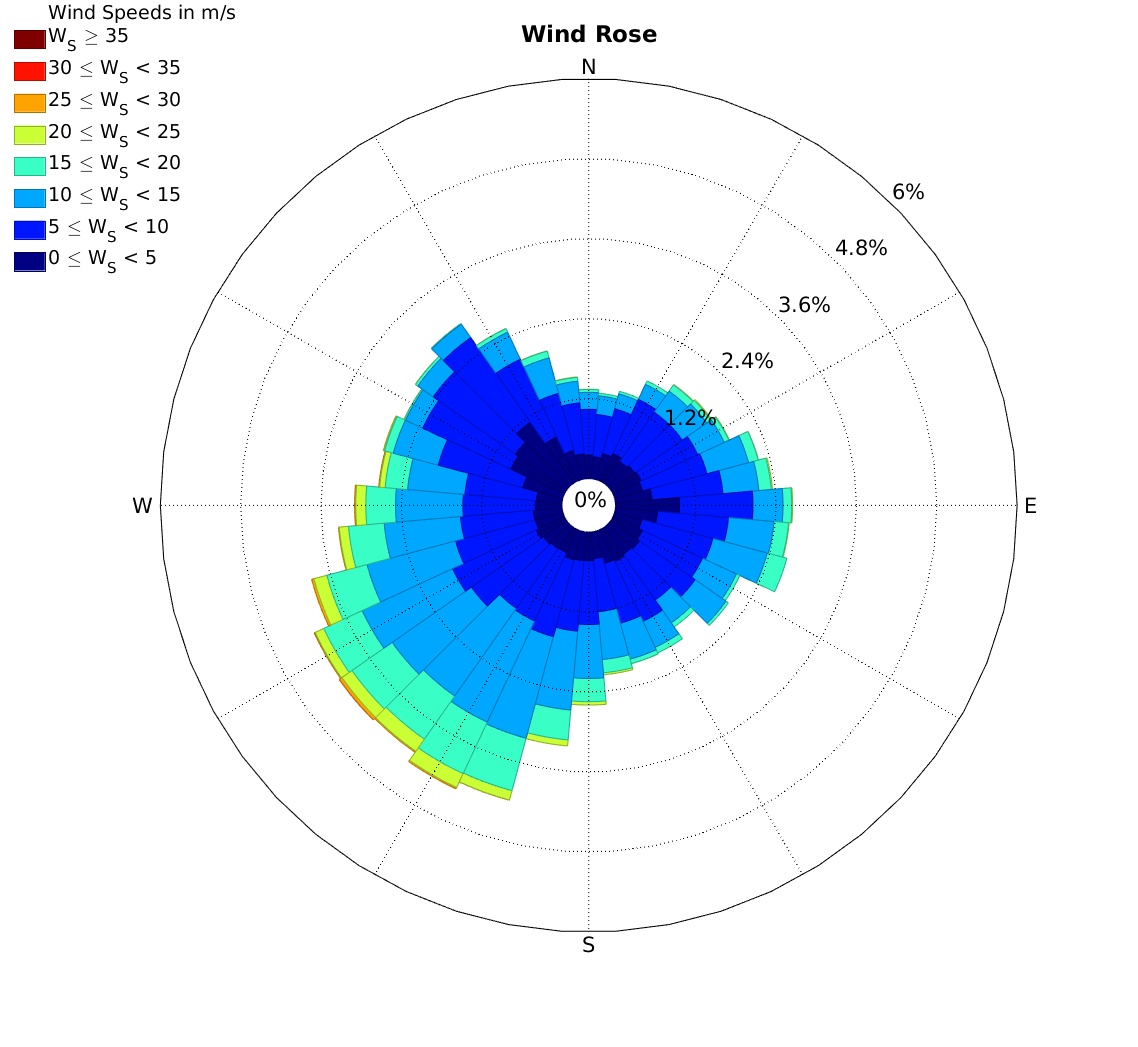
\includegraphics[width=1\linewidth]{../figures/WindRose_Fino1.png}
  \caption{Wind rose of FINO 1}
\end{subfigure}
\begin{subfigure}{0.58\textwidth}
  \centering
  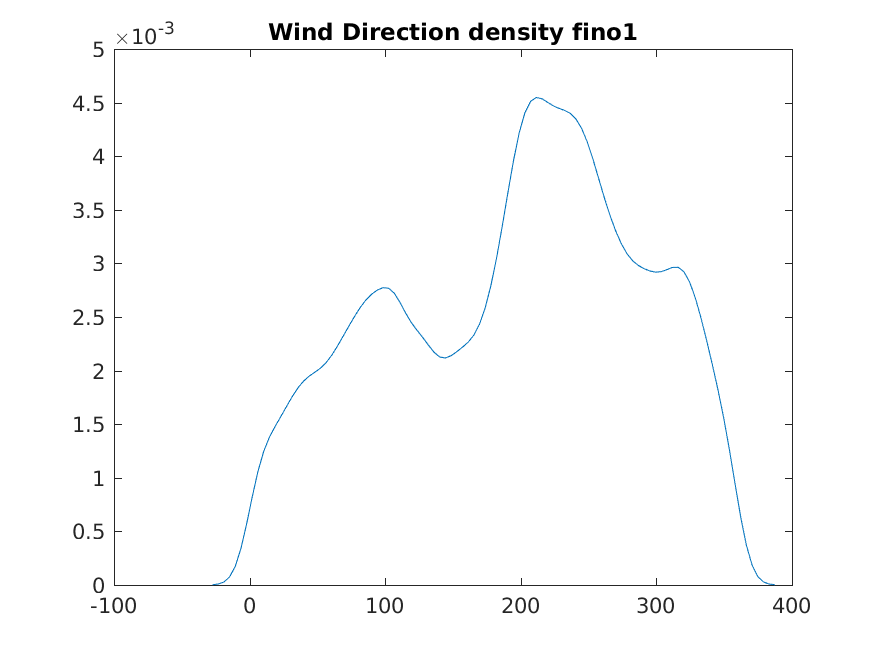
\includegraphics[width=1\linewidth]{../figures/Validation_WindRose_Fino1.png}
  \caption{pdf plot FINO 1}
\end{subfigure}
  \caption{Validation of Wind Rose}
\label{fig:WindroseValidation}
\end{figure}
\newpage
The pdf plot confirms that most of the wind is coming from south-west direction. This is identical with our FINO 1 wind rose. The same approach was used to confirm the wind rose created from FINO 2 data (see Appendix).
After validating our results we now can compare the two windroses. See Figure~\ref{fig:WindrosesVal}.

\begin{figure}[htb!]
\label{fig:WindRose1_valdidation}
\begin{subfigure}{0.5\textwidth}
  \centering
  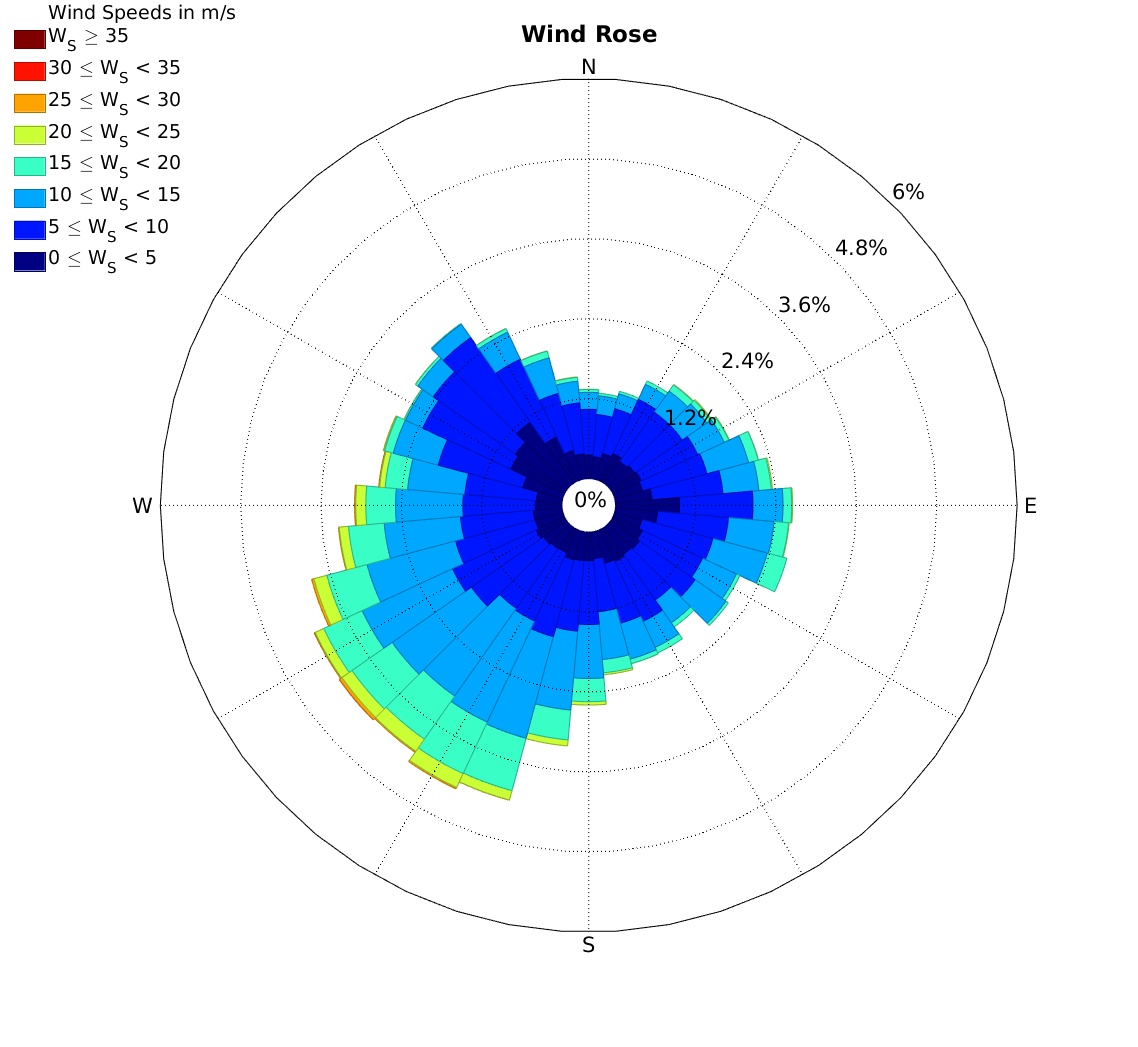
\includegraphics[width=1\linewidth]{../figures/WindRose_Fino1.png}
  \caption{Wind rose of FINO 1}
\end{subfigure}
\begin{subfigure}{0.5\textwidth}
  \centering
  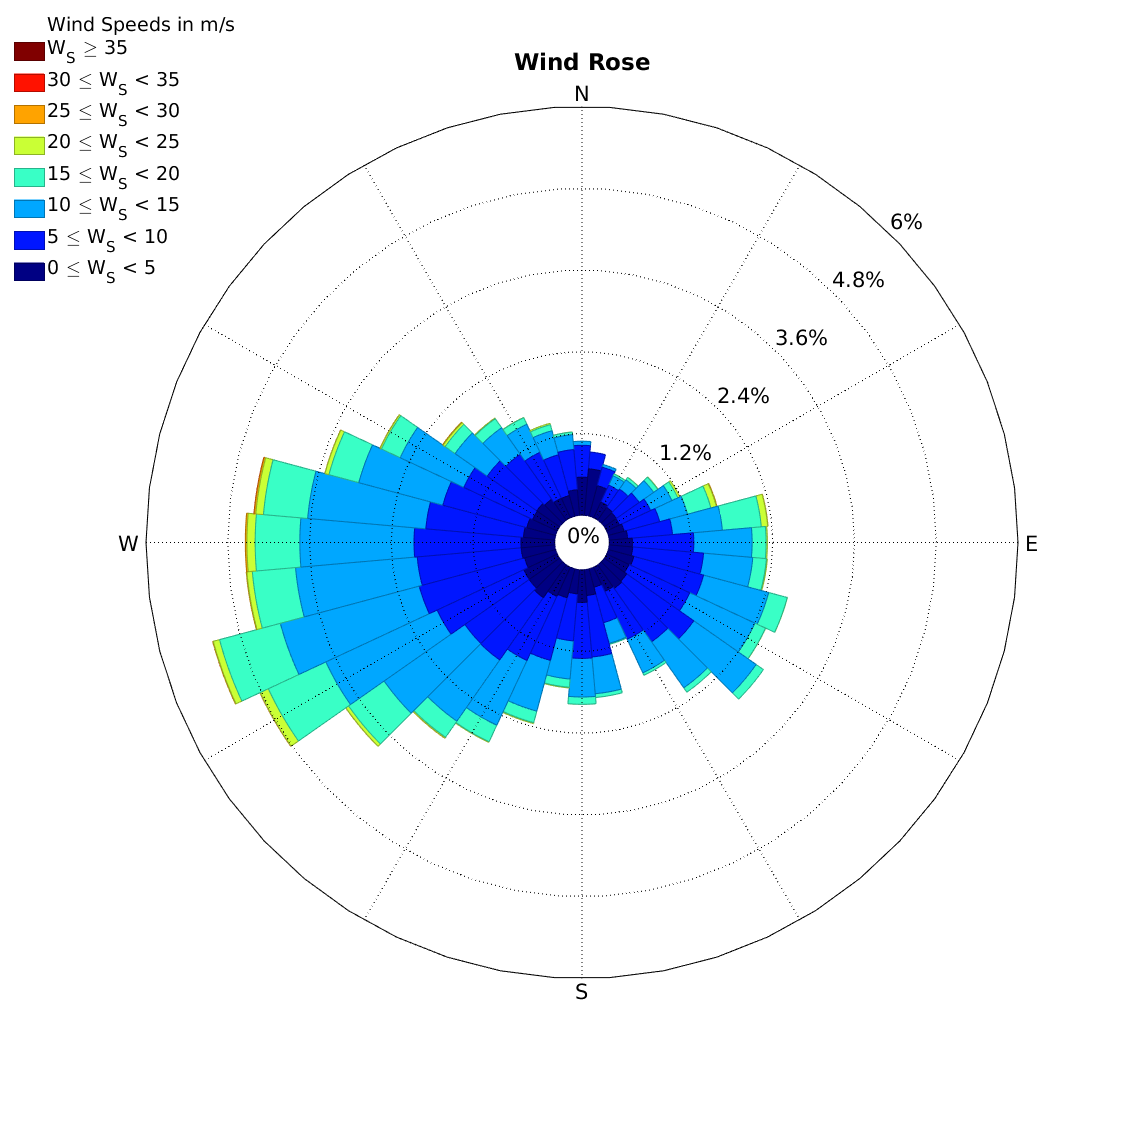
\includegraphics[width=1\linewidth]{../figures/WindRose_Fino2.png}
  \caption{Wind rose of FINO 2}
\end{subfigure}
\caption{Comparison of windroses}
  \label{fig:WindrosesVal}
\end{figure}
We observe that most of the measured wind directions at FINO 1 are of south-western direction. For FINO 2, located in the Baltic Sea, the wind is less distributed and has almost exclusively western and eastern directions. Both met masts are located in the Northern Hemisphere. That means high pressure fields rotate clockwise and low pressure fields anti-clockwise. The wind directions are influenced by the isobars of the different pressure fields. Keeping this information in mind and looking at the content provided during the lecture (see Figure~\ref{fig:weatherpattern}) the measured wind directions have two components. First the large scale wind movements are responsible for the south-western direction measured at FINO 1 and respectively western direction for FINO 2. The strong fluctuation in the lower wind speeds is due to the movement of the different pressure fields. Most of the time we have a high pressure field in the Baltic sea which might explain the additional components measured in eastern direction. For the north sea we observe an additional south western component.\\

\begin{figure}[H]
\centering
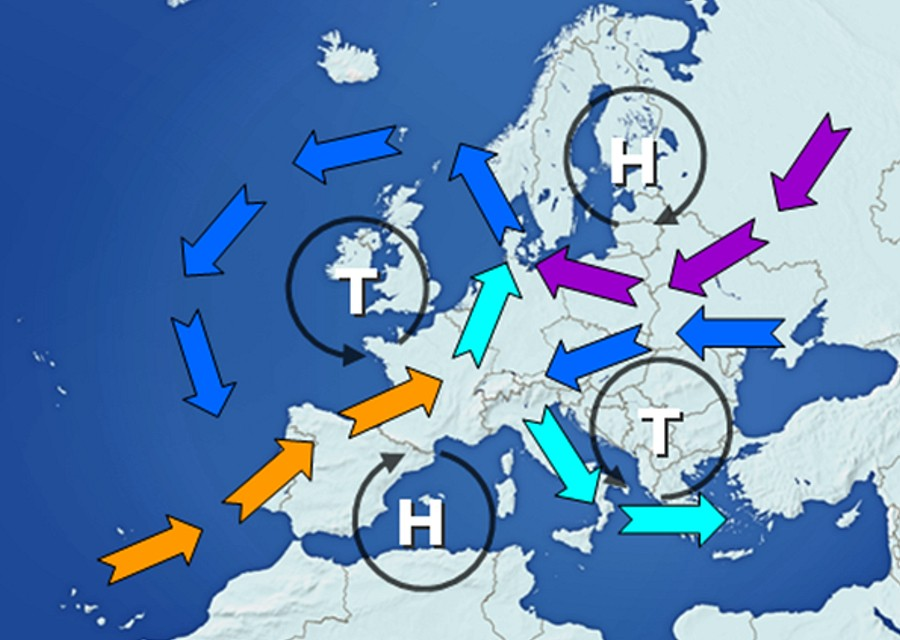
\includegraphics[width=0.5\linewidth]{../figures/warm_air_advection.png}
\caption{Typical weather pattern over Europe}
\label{fig:weatherpattern}
\end{figure}

Both measurement systems are located in the open sea, so in general there are no obstacles that can create additional turbulence. However the construction of wind farms may influence the measurement. This holds especially for FINO 1 which is nearly entirely surrounded by wind farms. (see Figure \ref{fig:fino1}).\\

\begin{figure}[H]
\centering
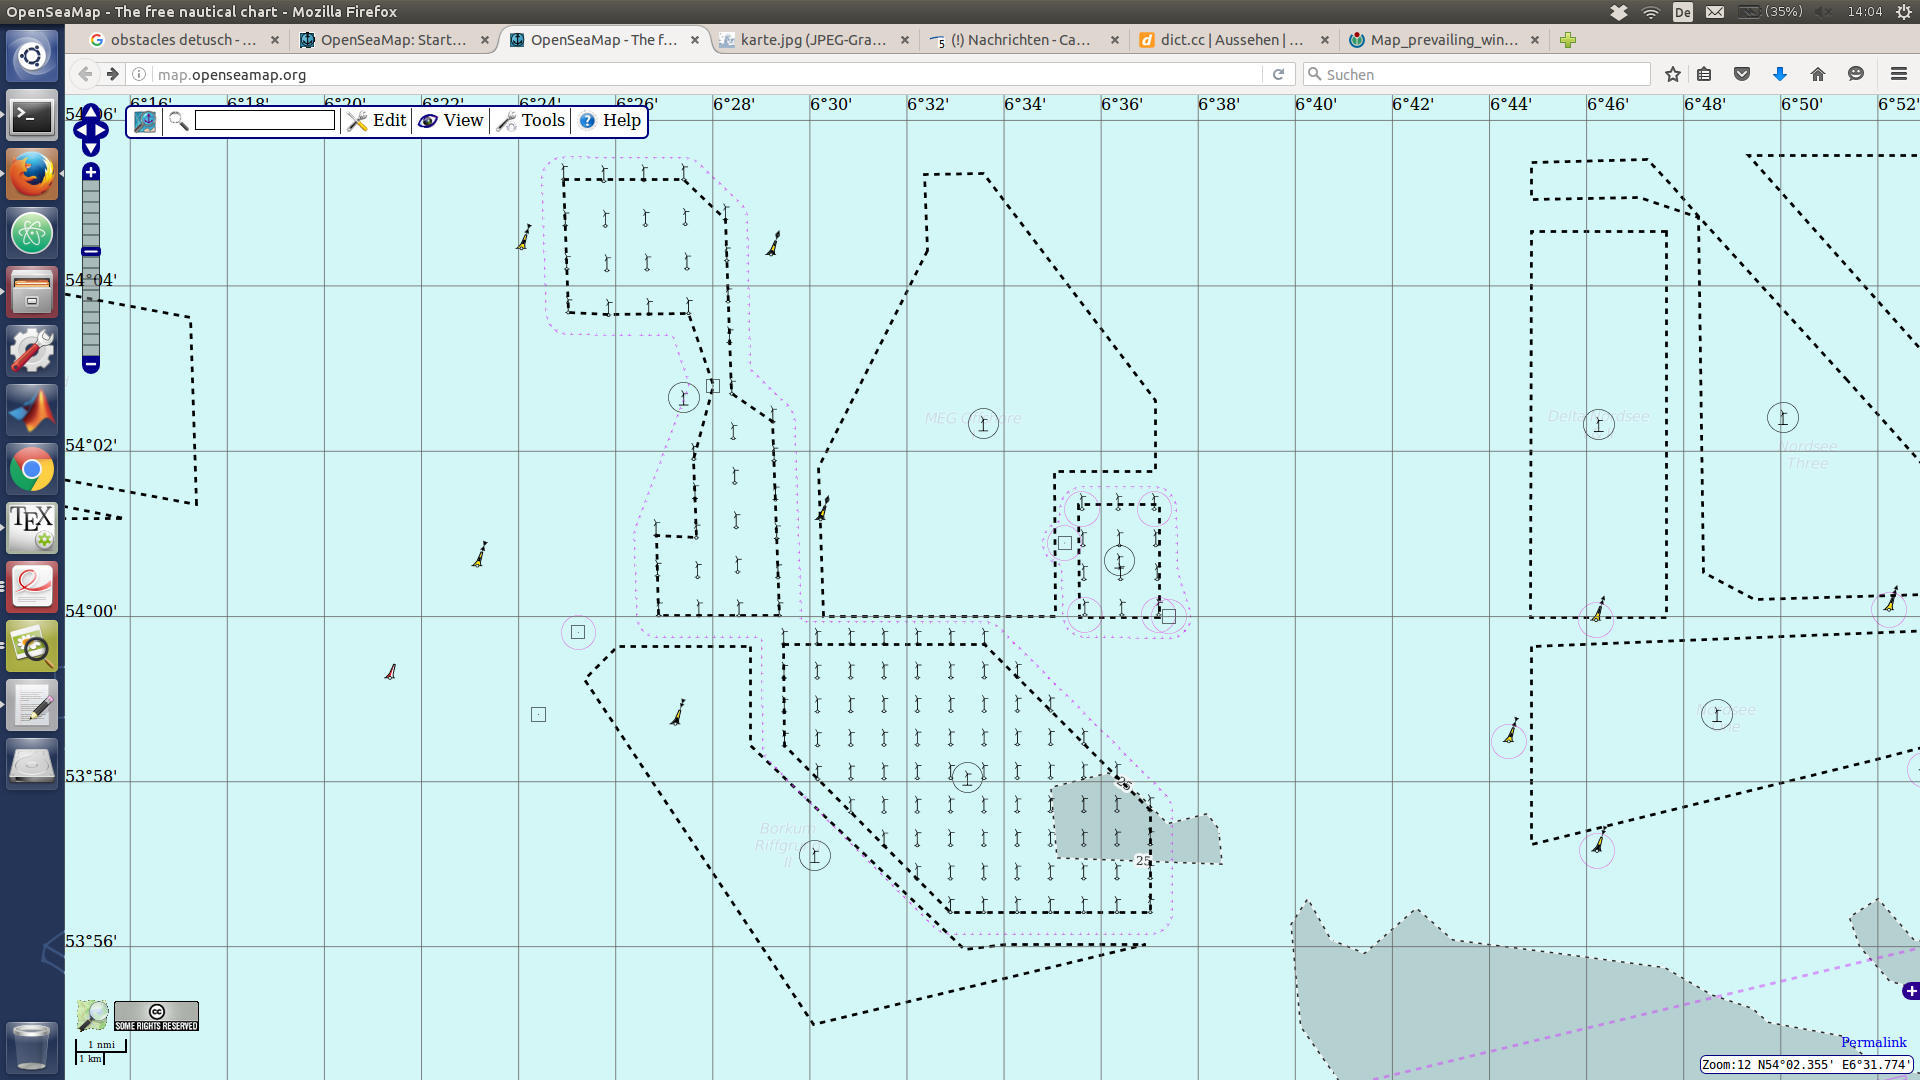
\includegraphics[width=0.5\linewidth]{../figures/fino1.png}
\caption{Location of FINO 1}
\label{fig:fino1}
\end{figure} 
 
\newpage
\section{Weibull distribution}
In Task 2 we created histograms at around $90m$ height. Next we calculated the Weibull parameters with the mean and standard deviation of the measured wind speeds. For the further calculation we used the equalities provided during the lecture:
\begin{align*}
&\mu = \lambda \cdot \Gamma\left(1+\frac{1}{k}\right) \\
&\sigma^2 = \lambda^2 \cdot \left(\Gamma\left(1+\frac{2}{k}\right)-\Gamma\left(1+\frac{1}{k}\right)^2\right)
\end{align*}
By substitution we obtain:
\begin{align*}
&\sigma^2 = \left(\frac{\mu}{\Gamma(1+\frac{1}{k})}\right)^2 \cdot \left(\Gamma\left({1+\frac{2}{k}}\right)-\Gamma\left(1+\frac{1}{k}\right)^2\right)
\end{align*}
which gives
\begin{align*}
&0 = \left(\frac{\mu}{\sigma}\right)^2 \cdot \left(\frac{\Gamma\left({1+\frac{2}{k}}\right)}{\Gamma\left(1+\frac{1}{k}\right)^2}-1\right)-1
\end{align*}
 We implemented this equation in Matlab and solved for the Weibull parameters A and k. With the calculated parameters we created a corresponding Weibull distribution.


\begin{lstlisting}
%% Task 2
mean1 = nanmean(fino1_v90);
dev1 = nanstd(fino1_v90);

mean2 = nanmean(fino2_v92);
dev2 = nanstd(fino2_v92);

% interpolate
k_Fino1 = 1;
Func_Fino1 = @(k_Fino1) (mean1*mean1/(dev1*dev1))*((gamma(1+2/k_Fino1))/(gamma(1+1/k_Fino1))^2-1)-1 
k_Fino1 = fsolve(Func_Fino1,k_Fino1);
disp(k_Fino1);
A_Fino1 = mean1/gamma(1+1/k_Fino1);
weibull_Fino1 = wblpdf(1:30,A_Fino1,k_Fino1);

k_Fino2 = 1;
Func_Fino2 = @(k_Fino2) (mean2*mean2/(dev2*dev2))*((gamma(1+2/k_Fino2))/(gamma(1+1/k_Fino2))^2-1)-1 
k_Fino2 = fsolve(Func_Fino2,k_Fino2);
disp(k_Fino2);
A_Fino2 = mean2/gamma(1+1/k_Fino2);
weibull_Fino2 = wblpdf(1:30,A_Fino2,k_Fino2);
\end{lstlisting}

Figure~\ref{fig:Histograms} shows the wind speed distributions for Fino 1 and Fino 2 with the corresponding Weibull fit.
\begin{figure}[H]
\begin{subfigure}{0.5\textwidth}
  \centering
  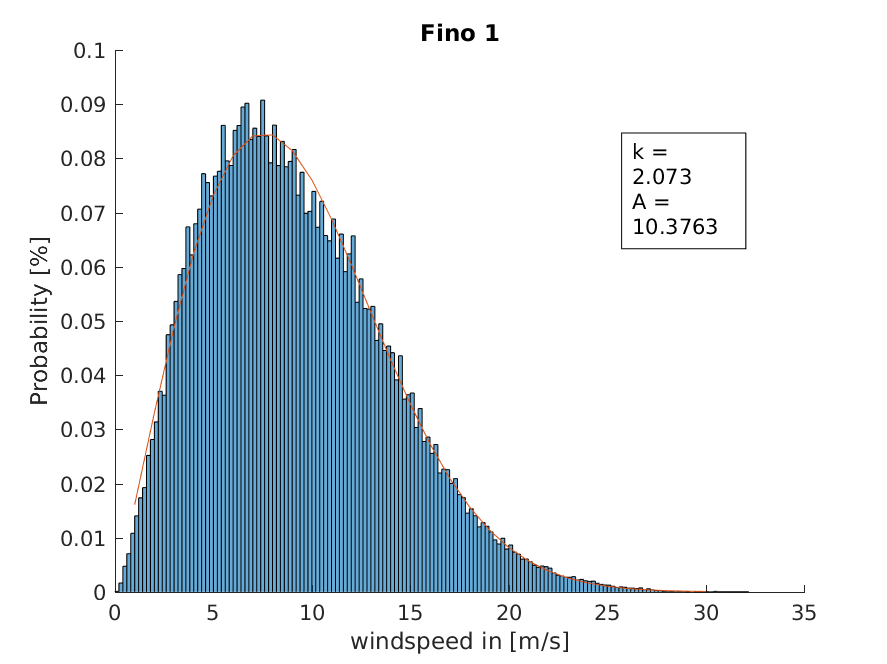
\includegraphics[width=1\linewidth]{../figures/Hist_withfit_Fino1.png}
  \caption{Histogram with Weibull fit FINO 1}
\end{subfigure}
\begin{subfigure}{0.5\textwidth}
  \centering
  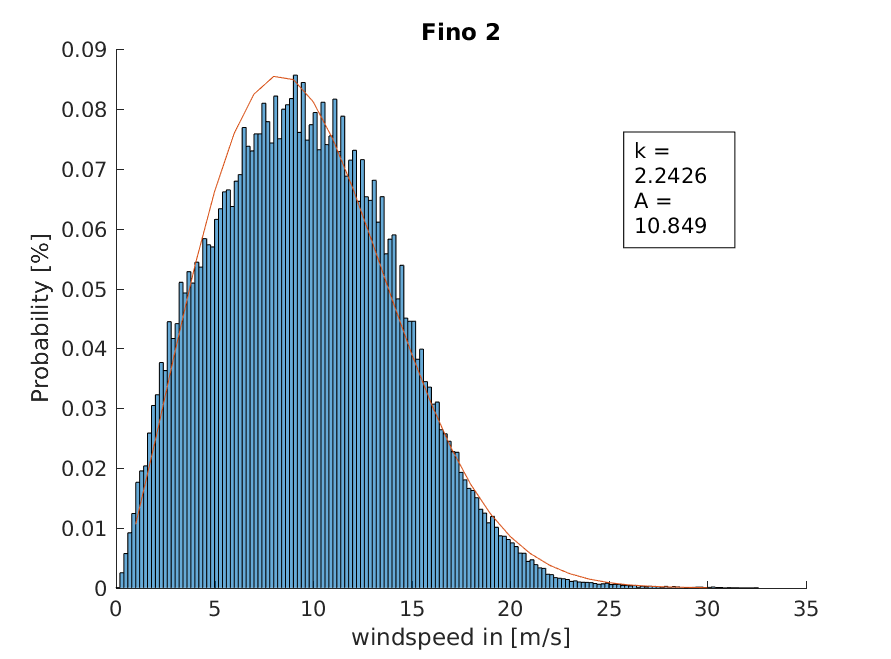
\includegraphics[width=1\linewidth]{../figures/Hist_withfit_Fino2.png}
  \caption{Histogram with Weibull fit FINO 2}
\end{subfigure}
  \caption{Wind speed distributions}
\label{fig:Histograms}
\end{figure}
In order to evaluate which region is more favorable for wind power utilization, we implemented two wind turbine power curves and calculated the energy yield.
The location of FINO 2 seems to be better for wind power utilization. This goes in hand with our first impression, because the curve of FINO 1 is a little shifted to the left hand side. However there are some concerns: The measured data might be influenced by the surrounding wind farms. The original wind speeds might be higher. In addition we only evaluated one height. We have not included measurements at different heights. We just assume that we have a comparable vertical wind speed distribution. 
\newpage

\section{Vertical wind profiles}
In the following task we calculated the vertical wind speed profile for the wind sector in the range of $240 - 285$ degrees. In the lecture we discussed two common methods for the vertical wind profile: the empirical power law profile and the logarithmic wind speed profile. We were asked to fit these methods to our data. The following code snippet shows how we implemented the fitting routine in Matlab:

\begin{lstlisting}
logProfileModel = @(b,z) b(1)/0.4 *(log(z/b(2)));
empPowerModel = @(c,x) avgPerHeight(8)*((x/90).^c(1));
opts = statset('nlinfit');
opts.RobustWgtFun = 'bisquare';
logProfileCoeffs = nlinfit([33,40,50,60,70,80,90,100],avgPerHeight,logProfileModel,[0.2,10^-6],opts);
[x,y]=fplot(@(z) logProfileCoeffs(1)/0.4 *(log(z/logProfileCoeffs(2))),[0 100]);
plot(y,x,'Color','b');
empPowerCoeff = real(nlinfit([33,40,50,60,70,80,90,100],avgPerHeight,empPowerModel,[0.11],opts));
[x,y]=fplot(@(z) avgPerHeight(8)*(z/90)^(empPowerCoeff),[0 100]);
plot(y,x,'Color','r');
\end{lstlisting}

Figure \ref{fig:verticalfit} shows the result of our fitting.

\begin{figure}[H]
\centering
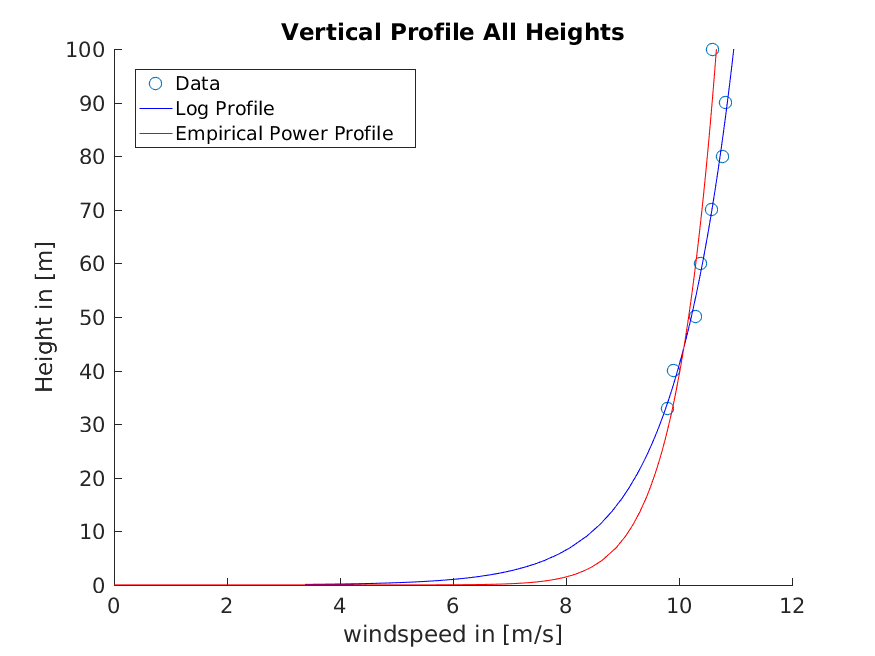
\includegraphics[width=0.7\linewidth]{../figures/verticalProfileFits.png}
\caption{Vertical profile fits}
\label{fig:verticalfit}
\end{figure}

The figure shows the data points, calculated by the mean wind speed of the different heights and the corresponding logarithmic and empirical power law profile.
Our results suggest that the logarithmic profile is more accurate for the given data. The power law profile has a stronger gradient and is especially different for low wind speeds. While the logarithmic model fits most of the data points quite well (except $z=100m$) the power law model fits the extreme values better. In this case we would thus prefer the logarithmic model because we consider the data point at $100m$ as a non-physical measurement error (e.g. defect anemometer at that height during one winter). However we cannot check which method is better for lower wind speeds. As starting values for the non-linear regression we chose $u_{*}=0.2$ for the friction velocity and $z_0 = 10^{-6}$ for the roughness length in the logarithmic model and $\alpha=0.11$ for the power law model according to the lecture notes recommending these values in case of water surface.
The two regressions end with the following values:
\begin{align*}
&u_{*}= 0.434\\
&z_0 = 0.0041\\
&\alpha = 0.0682
\end{align*}
\newpage

\section{Seasonal aspects of the vertical wind profile}
In the extra task (3b) we were to study seasonal aspects of the vertical wind speed profile by comparing the vertical profile during summer time (May-July) with winter time (November-January). For both seasons we considered western/south-western winds again in the range of $240 - 285$ degrees. For both seasons we performed a non-linear regression again with the logarithmic model and the power law model. Results for this are depicted in Figure~\ref{fig:seasonalProfiles}.

\begin{figure}[H]
\begin{subfigure}{0.5\textwidth}
  \centering
  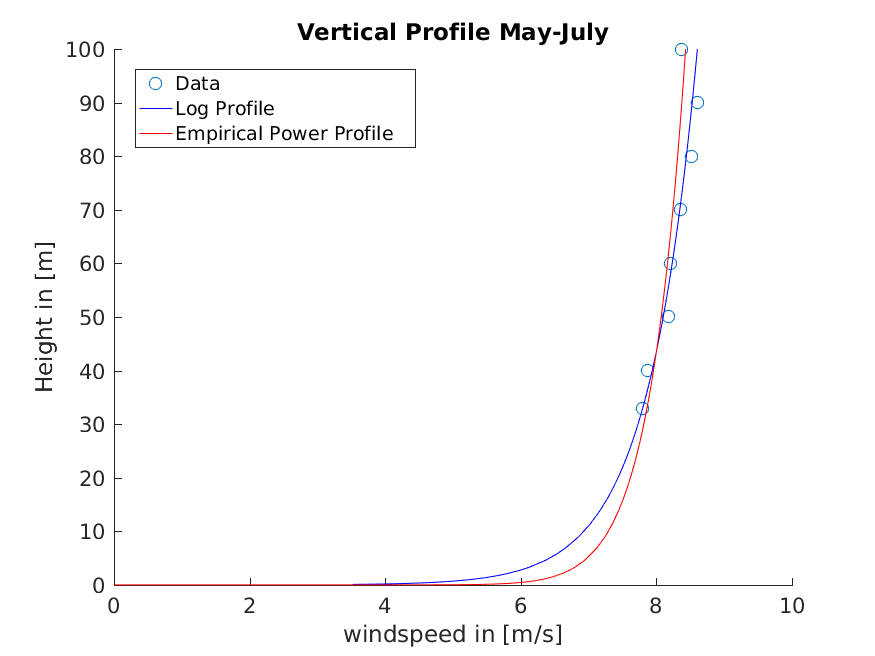
\includegraphics[width=1\linewidth]{../figures/verticalProfileFitsSommer.png}
  \caption{May-July}
\end{subfigure}
\begin{subfigure}{0.5\textwidth}
  \centering
  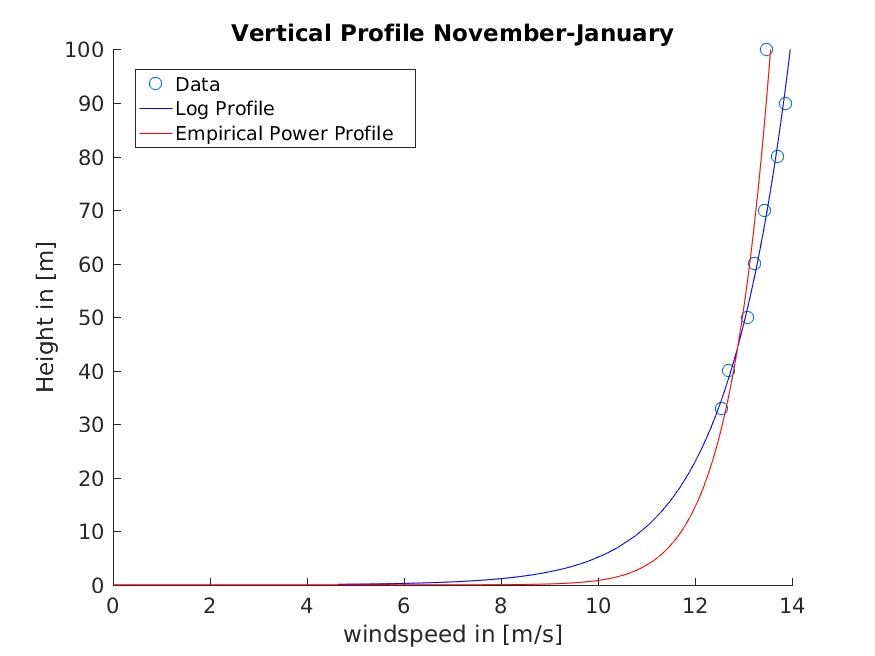
\includegraphics[width=1\linewidth]{../figures/verticalProfileFitsWinter.png}
  \caption{November-January}
\end{subfigure}
  \caption{vertical profiles in summer and winter}
\label{fig:seasonalProfiles}
\end{figure}

Not surprisingly the overall wind speed is higher in winter. But from this graphic the shape of the curves are very much similar with regard to the vertical profile. In order to detect differences we normalized the model curves to a wind speed of $1$ at height $z=90$. By doing so we can state that the vertical wind speed profile during summer is clearly steeper (red dashed curve in Figure~\ref{fig:verticalProfComp}) than in winter (blue dashed curve) regarding the logarithmic regression model. 

\begin{figure}[H]
\centering
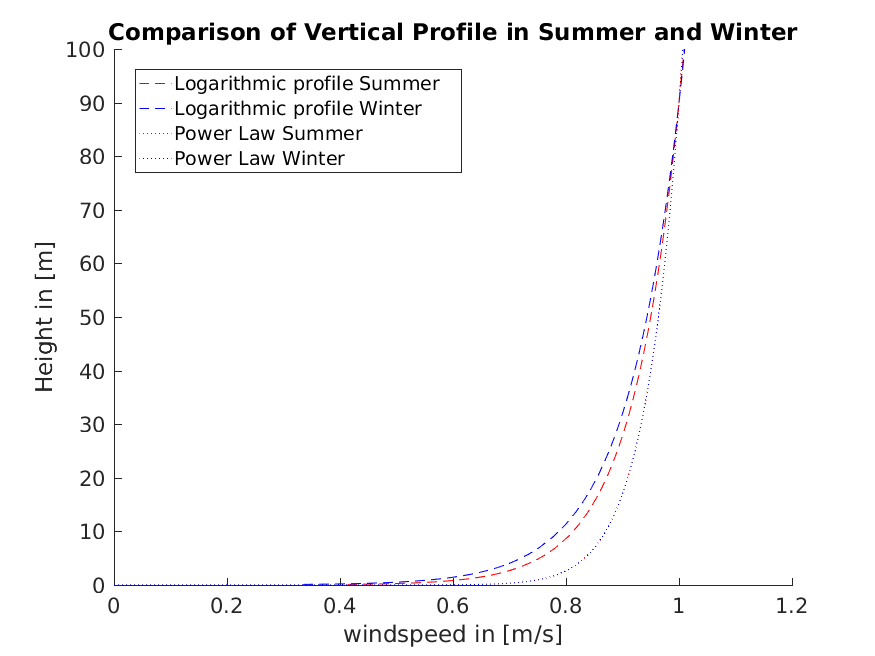
\includegraphics[width=0.7\linewidth]{../figures/verticalProfilesComparison.png}
\caption{Vertical profile fits}
\label{fig:verticalProfComp}
\end{figure}

This means that the wind shear in summer time is lower compared to the wind shear in winter. In the empirical power law model this difference does not hold (the curves for summer and winter are identical). However, as stated previously we consider the logarithmic model to be more accurate and reason that the seasonal variation in vertical wind shear is due to more turbulent and overall higher winds with higher waves in winter while summer sees more steady and constant wind.
We can make this observation even more obvious by looking at the final values of the variables in the logarithmic regression model. In summer the regression ends with values of $v_{*}=0.2906$ and $z_0=0.0007$ while in winter we obtain $v_{*}=0.5338$ and $z_0=0.0029$. Thus the friction velocity and the surface roughness are almost doubled in winter which accounts for the higher vertical wind shear. \\

\newpage

\appendix
\section{Appendix}
\subsection{Task 1}
\begin{figure}[H]
\begin{subfigure}{0.5\textwidth}
  \centering
  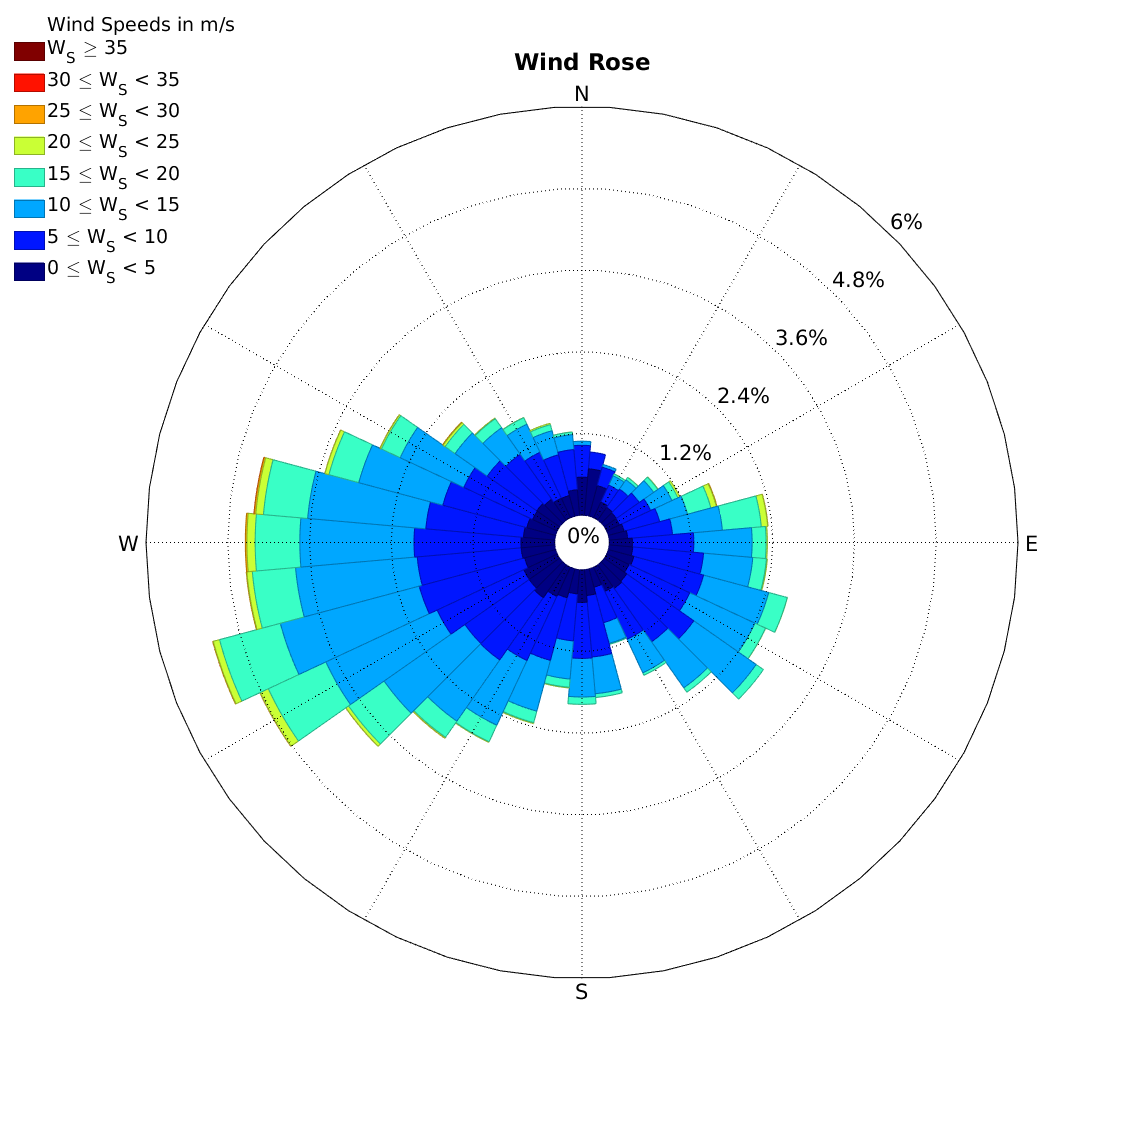
\includegraphics[width=1\linewidth]{../figures/WindRose_Fino2.png}
  \caption{Wind rose of FINO 2}
\end{subfigure}
\begin{subfigure}{0.5\textwidth}
  \centering
  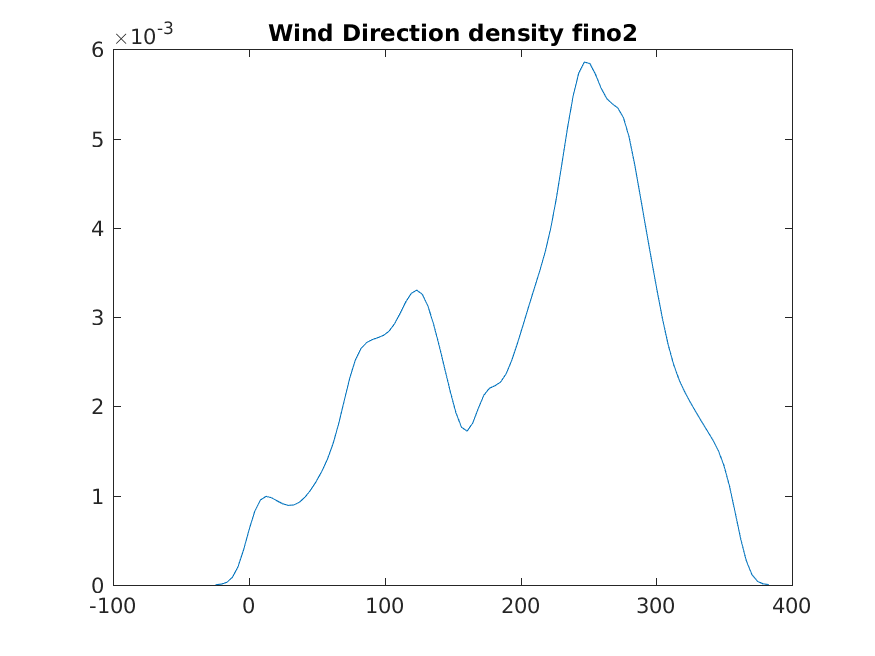
\includegraphics[width=1\linewidth]{../figures/Validation_WindRose_Fino2.png}
  \caption{pdf plot FINO 2}
\end{subfigure}
  \caption{Validation of Wind Rose 2}
\label{fig:WindroseValidation2}
\end{figure}

\subsection{Code}
\begin{lstlisting}
%% Task 1
disp('Load Data')
load('WMP_WEnMet_data.mat');

fino1_v90 = Fino1.ws90;
fino1_d90 = Fino1.wd90;
fino2_v92 = Fino2.ws92;
fino2_d91 = Fino2.wd91;

% Plot
WindRose(fino1_d90,fino1_v90,'AngleNorth',0,'AngleEast',90);
saveas(gcf,'figures/WindRose_Fino1.png')
WindRose(fino2_d91,fino2_v92,'AngleNorth',0,'AngleEast',90);
saveas(gcf,'figures/WindRose_Fino2.png')


% Validate wind rose ...
[a,b] = ksdensity(fino2_d91)
figure();
plot(b,a)
title('Wind Direction density fino2')
saveas(gcf,'figures/Validation_WindRose_Fino2.png')
[c,d] = ksdensity(fino1_d90)
figure();
plot(d,c)
title('Wind Direction density fino1')
saveas(gcf,'figures/Validation_WindRose_Fino1.png')

%% Task 2
mean1 = nanmean(fino1_v90);
dev1 = nanstd(fino1_v90);

mean2 = nanmean(fino2_v92);
dev2 = nanstd(fino2_v92);

% interpolate
k_Fino1 = 2.073;
Func_Fino1 = @(k_Fino1) (mean1*mean1/(dev1*dev1))*((gamma(1+2/k_Fino1))/(gamma(1+1/k_Fino1))^2-1)-1 
k_Fino1 = fsolve(Func_Fino1,k_Fino1);
disp(k_Fino1);
A_Fino1 = mean1/gamma(1+1/k_Fino1);
weibull_Fino1 = wblpdf(1:30,A_Fino1,k_Fino1);

k_Fino2 = 2.2426;
Func_Fino2 = @(k_Fino2) (mean2*mean2/(dev2*dev2))*((gamma(1+2/k_Fino2))/(gamma(1+1/k_Fino2))^2-1)-1 
k_Fino2 = fsolve(Func_Fino2,k_Fino2);
disp(k_Fino2);
A_Fino2 = mean2/gamma(1+1/k_Fino2);
weibull_Fino2 = wblpdf(1:30,A_Fino2,k_Fino2);


x_vestas = (0:25)';
y_vestas = [0, 0,0,0,91,200,362,588,889,1255,1604,1769,1798,1800,1800,1800,1800,1800,1800,1800,1800,1800,1800,1800,1800,1800]';

x_enercon = (0:25)';
y_enercon = [0,0,3,25,82,174,321,532,815,1180,1580,1900,2200,2400,2480,2700,2850,2950,3020,3020,3020,3020,3020,3020,3020,3020]';

for i = 1:25
    fino1_vestasyield(i,1) = y_vestas(i)*weibull_Fino1(i);
    fino2_vestasyield(i,1) = y_vestas(i)*weibull_Fino2(i);
    fino1_enerconyield(i,1) = y_enercon(i)*weibull_Fino1(i);
    fino2_enerconyield(i,1) = y_enercon(i)*weibull_Fino2(i);
end

if sum(fino1_vestasyield) > sum(fino2_vestasyield)
    disp('Fino 1 besser, vestas')
else
    disp('Fino 2 besser, vestas')
end

if sum(fino1_enerconyield) > sum(fino2_enerconyield)
    disp('Fino 1 besser, enercon')
else
    disp('Fino 2 besser, enercon')
end
 
figure();
hold on;
histogram(fino1_v90, 'Normalization', 'pdf');
plot(weibull_Fino1)
xlabel('windspeed in [m/s]');
ylabel('Probability [%]');
title('Fino 1')
dim = [.7 .5 .3 .3];
annotation('textbox',dim,'String',{'k =',num2str(k_Fino1), 'A =' ,num2str(A_Fino1)},'FitBoxToText','on');
saveas(gcf,'figures/Hist_withfit_Fino1.png')
hold off;

figure();
hold on;
histogram(fino2_v92, 'Normalization', 'pdf');
plot(weibull_Fino2)
xlabel('windspeed in [m/s]');
ylabel('Probability [%]');
title('Fino 2')
dim = [.7 .5 .3 .3];
annotation('textbox',dim,'String',{'k =',num2str(k_Fino2), 'A =' ,num2str(A_Fino2)},'FitBoxToText','on');
saveas(gcf,'figures/Hist_withfit_Fino2.png')
hold off;

%% Task 3
wind_sector = [];
windsOnHeight = [];
j = 1
for i = 1:length(fino1_v90)
    if (fino1_d90(i) >= 240 && fino1_d90(i) <= 285)
        wind_sector(j,2) = fino1_v90(1,i);
        wind_sector(j,1) = fino1_d90(1,i);
        windsOnHeight(j,1) = Fino1.ws33(1,i);
        windsOnHeight(j,2) = Fino1.ws40(1,i);
        windsOnHeight(j,3) = Fino1.ws50(1,i);
        windsOnHeight(j,4) = Fino1.ws60(1,i);
        windsOnHeight(j,5) = Fino1.ws70(1,i);
        windsOnHeight(j,6) = Fino1.ws80(1,i);
        windsOnHeight(j,7) = Fino1.ws90(1,i);
        windsOnHeight(j,8) = Fino1.ws100(1,i);
        j= j+1;
    end
end

wind_sector_mean = nanmean(wind_sector(:,2));
wind_prof = [];
for i = 1:100
    wind_prof(i,1) = 0.2/0.4 *(log(i/10^-6));
    wind_prof(i,2) = wind_sector_mean*(i/90)^(0.11);
end
figure();
hold on;
plot(1:100, wind_prof(:,1))
plot(1:100,wind_prof(:,2), 'o')
plot(90,wind_sector_mean,'*')
xlabel('Height in [m]');
ylabel('windspeed in [m/s]');
title('Vertical Profile');

avgPerHeight = [8];
for i=1:8
   avgPerHeight(i) = nanmean(windsOnHeight(:,i));
end
figure();
hold on;
plot(avgPerHeight(:),[33,40,50,60,70,80,90,100], 'o')

logProfileModel = @(b,z) b(1)/0.4 *(log(z/b(2)));
empPowerModel = @(c,x) avgPerHeight(8)*((x/90).^c(1));
opts = statset('nlinfit');
opts.RobustWgtFun = 'bisquare';
logProfileCoeffs = nlinfit([33,40,50,60,70,80,90,100],avgPerHeight,logProfileModel,[0.2,10^-6],opts);
[x,y]=fplot(@(z) logProfileCoeffs(1)/0.4 *(log(z/logProfileCoeffs(2))),[0 100]);
plot(y,x,'Color','b');
empPowerCoeff = real(nlinfit([33,40,50,60,70,80,90,100],avgPerHeight,empPowerModel,[0.11],opts));
[x,y]=fplot(@(z) avgPerHeight(8)*(z/90)^(empPowerCoeff),[0 100]);
plot(y,x,'Color','r');

ylabel('Height in [m]');
xlabel('windspeed in [m/s]');
title('Vertical Profile All Heights');
legend('Data', 'Log Profile','Empirical Power Profile','Location','northwest');
saveas(gcf,'figures/verticalProfileFits.png')
hold off;

%% ExtraTask 3(b)

windsOnHeightSommer = [];
windsOnHeightWinter = [];
jS = 1
jW = 1

for i = 1:length(fino1_v90)
    if (fino1_d90(i) >= 240 && fino1_d90(i) <= 285) 
        if  ((i>6*24*(31+28+31+30) && i<=6*24*(31+28+31+30+31+30+31)) ... %May-July 2010
            || (i>6*24*(31+28+31+30+365) && i<=6*24*(31+28+31+30+31+30+31+365)) ... %May-July 2011
            || (i>6*24*(31+29+31+30+365+365) && i<=6*24*(31+29+31+30+31+30+31+365+365)) ... %May-July 2012
            || (i>6*24*(31+28+31+30+365+365+366) && i<=6*24*(31+28+31+30+31+30+31+365+365+366)) ... %May-July 2013
            || (i>6*24*(31+28+31+30+365+365+366+365) && i<=6*24*(31+28+31+30+31+30+31+365+365+366+365)) ... %May-July 2014
            || (i>6*24*(31+28+31+30+365+365+366+365+365) && i<=6*24*(31+28+31+30+31+30+31+365+365+366+365+365))) %May-July 2015
                windsOnHeightSommer(jS,1) = Fino1.ws33(1,i);
                windsOnHeightSommer(jS,2) = Fino1.ws40(1,i);
                windsOnHeightSommer(jS,3) = Fino1.ws50(1,i);
                windsOnHeightSommer(jS,4) = Fino1.ws60(1,i);
                windsOnHeightSommer(jS,5) = Fino1.ws70(1,i);
                windsOnHeightSommer(jS,6) = Fino1.ws80(1,i);
                windsOnHeightSommer(jS,7) = Fino1.ws90(1,i);
                windsOnHeightSommer(jS,8) = Fino1.ws100(1,i);
                jS= jS+1;
        end
         if ((i>0 && i<=6*24*31) ... %January 2010
            || (i>6*24*(365-31-30) && i<=6*24*(365+31)) ... %Nov2010-Jan2011
            || (i>6*24*(365+365-31-30) && i<=6*24*(365+365+31)) ... %Nov2011-Jan2012
            || (i>6*24*(365+365+366-31-30) && i<=6*24*(365+365+366+31)) ... %Nov2012-Jan2013
            || (i>6*24*(365+365+366+365-31-30) && i<=6*24*(365+365+366+365+31)) ... %Nov2013-Jan2014
            || (i>6*24*(365+365+366+365+365-31-30) && i<=6*24*(365+365+366+365+365+31)) ... %Nov2014-Jan2015
            || (i>6*24*(365+365+366+365+365+365-31-30) && i<=6*24*(365+365+366+365+365+365)+1)) %Nov2015-Dez2015
                windsOnHeightWinter(jW,1) = Fino1.ws33(1,i);
                windsOnHeightWinter(jW,2) = Fino1.ws40(1,i);
                windsOnHeightWinter(jW,3) = Fino1.ws50(1,i);
                windsOnHeightWinter(jW,4) = Fino1.ws60(1,i);
                windsOnHeightWinter(jW,5) = Fino1.ws70(1,i);
                windsOnHeightWinter(jW,6) = Fino1.ws80(1,i);
                windsOnHeightWinter(jW,7) = Fino1.ws90(1,i);
                windsOnHeightWinter(jW,8) = Fino1.ws100(1,i);
                jW= jW+1;
        end
    end
end

%Evaluation of Sommer Months 2010-2015
avgPerHeightSommer = [8];
for i=1:8
   avgPerHeightSommer(i) = nanmean(windsOnHeightSommer(:,i));
end
figure();
hold on;
plot(avgPerHeightSommer(:),[33,40,50,60,70,80,90,100], 'o')

logProfileModel = @(b,z) b(1)/0.4 *(log(z/b(2)));
empPowerModel = @(c,z) avgPerHeightSommer(8)*((z/90).^c(1));
opts = statset('nlinfit');
opts.RobustWgtFun = 'bisquare';
logProfileCoeffsSom = nlinfit([33,40,50,60,70,80,90,100],avgPerHeightSommer,logProfileModel,[0.2,10^-6],opts);
[xLogSom,yLogSom]=fplot(@(z) logProfileCoeffsSom(1)/0.4 *(log(z/logProfileCoeffsSom(2))),[0 100]);
plot(yLogSom,xLogSom,'Color','b');
empPowerCoeffSom = nlinfit([33,40,50,60,70,80,90,100],avgPerHeightSommer,empPowerModel,[0.11],opts);
[xPowSom,yPowSom]=fplot(@(z) avgPerHeightSommer(8)*(z/90)^(empPowerCoeffSom),[0 100]);
plot(yPowSom,xPowSom,'Color','r');

ylabel('Height in [m]');
xlabel('windspeed in [m/s]');
title('Vertical Profile May-July');
legend('Data', 'Log Profile','Empirical Power Profile','Location','northwest');
saveas(gcf,'figures/verticalProfileFitsSommer.png')
hold off;

%Evaluation of Winter Months 2010-2015
avgPerHeightWinter = [8];
for i=1:8
   avgPerHeightWinter(i) = nanmean(windsOnHeightWinter(:,i));
end
figure();
hold on;
plot(avgPerHeightWinter(:),[33,40,50,60,70,80,90,100], 'o')

logProfileModelWin = @(b,z) b(1)/0.4 *(log(z/b(2)));
empPowerModelWin = @(c,z) avgPerHeightWinter(8)*((z/90).^c(1));
opts = statset('nlinfit');
opts.RobustWgtFun = 'bisquare';
logProfileCoeffsWin = real(nlinfit([33,40,50,60,70,80,90,100],avgPerHeightWinter,logProfileModelWin,[0.1,10^-5],opts));
[xLogWin,yLogWin]=fplot(@(z) logProfileCoeffsWin(1)/0.4 *(log(z/logProfileCoeffsWin(2))),[0 100]);
plot(yLogWin,xLogWin,'Color','b');
empPowerCoeffWin = nlinfit([33,40,50,60,70,80,90,100],avgPerHeightWinter,empPowerModelWin,0.063,opts);
[xPowWin,yPowWin]=fplot(@(z) avgPerHeightWinter(8)*(z/90)^(empPowerCoeffWin),[0 100]);
plot(yPowWin,xPowWin,'Color','r');

ylabel('Height in [m]');
xlabel('windspeed in [m/s]');
title('Vertical Profile November-January');
legend('Data', 'Log Profile','Empirical Power Profile','Location','northwest');
saveas(gcf,'figures/verticalProfileFitsWinter.png')
hold off;

%comparison of normed log profiles in summer and winter
figure();
hold on;
yLogSomNormed = yLogSom/logProfileModel(logProfileCoeffsSom,90);
yLogWinNormed = yLogWin/logProfileModelWin(logProfileCoeffsWin,90);
plot(yLogSomNormed,xLogSom,'--','Color','r');
plot(yLogWinNormed,xLogWin,'--','Color','b');

yPowSomNormed = yPowSom/empPowerModel(empPowerCoeffSom,90);
yPowWinNormed = yPowWin/empPowerModelWin(empPowerCoeffWin,90);

plot(yPowSomNormed,xPowSom,':','Color','r');
plot(yPowWinNormed,xPowWin,':','Color','b');
ylabel('Height in [m]');
xlabel('windspeed in [m/s]');
title('Comparison of Vertical Profile in Summer and Winter');
legend('Logarithmic profile Summer', 'Logarithmic profile Winter','Power Law Summer','Power Law Winter','Location','northwest');
saveas(gcf,'figures/verticalProfilesComparison.png')
hold off;

disp(logProfileCoeffsSom);
disp(empPowerCoeffSom);
disp(logProfileCoeffsWin);
disp(empPowerCoeffWin);

\end{lstlisting}
\end{document}